%%%%%%%%%%%%%%%%%%%%%%%%%%%%%%%%%%%%%%%%%
% The Legrand Orange Book
% LaTeX Template
% Version 3.1 (February 18, 2022)
% Compiling this template:
% This template uses biber for its bibliography and makeindex for its index.
% When you first open the template, compile it from the command line with the 
% commands below to make sure your LaTeX distribution is configured correctly:
%
% 1) pdflatex mainv2
% 2) makeindex mainv2.idx -s indexstyle.ist
% 3) biber mainv2
% 4) pdflatex mainv2 x 2


%Atención
%Está prohibido usar simbolos en \index{•}
% After this, when you wish to update the bibliography/index use the appropriate
% command above and make sure to compile with pdflatex several times 
% afterwards to propagate your changes to the document.
%
%%%%%%%%%%%%%%%%%%%%%%%%%%%%%%%%%%%%%%%%%

%----------------------------------------------------------------------------------------
%	PACKAGES AND OTHER DOCUMENT CONFIGURATIONS
%----------------------------------------------------------------------------------------

\documentclass[
	12pt, % Default font size, select one of 10pt, 11pt or 12pt
	fleqn, % Left align equations
	a4paper, % Paper size, use either 'a4paper' for A4 size or 'letterpaper' for US letter size
	oneside, % Uncomment for oneside mode, this doesn't start new chapters and parts on odd pages (adding an empty page if required), this mode is more suitable if the book is to be read on a screen instead of printed
]{LegrandOrangeBook}

% Book information for PDF metadata, remove/comment this block if not required 
\hypersetup{
	pdftitle={Apuntes sobre las Telecomunicaciones}, % Title field
	pdfauthor={Jose Hancco}, % Author field
	pdfsubject={Educación}, % Subject field
	pdfkeywords={Telecomunicaciones, UNSA, Pregrado, Señales}, % Keywords
	pdfcreator={LaTeX}, % Content creator field
}

\addbibresource{sample.bib} % Bibliography file

\definecolor{ocre}{RGB}{63, 76, 83} % Define the color used for highlighting throughout the book, replace it with average color for a better presentation:
% Background.pdf -> Average color=63,76,83
% Background1.pdf -> Average color=31,31,40
% Background2.pdf -> Average color=123,119,101
% Background3.pdf -> Average color=103,61,76
\chapterimage{Final1.jpg} % Chapter heading image
\chapterspaceabove{6.5cm} % Default whitespace from the top of the page to the chapter title on chapter pages
\chapterspacebelow{6.75cm} % Default amount of vertical whitespace from the top margin to the start of the text on chapter pages

%----------------------------------------------------------------------------------------

\begin{document}

%----------------------------------------------------------------------------------------
%	TITLE PAGE
%----------------------------------------------------------------------------------------

\begingroup
\thispagestyle{empty} % Suppress headers and footers on the title page
\begin{tikzpicture}[remember picture,overlay]
\node[inner sep=0pt] (background) at (current page.center) {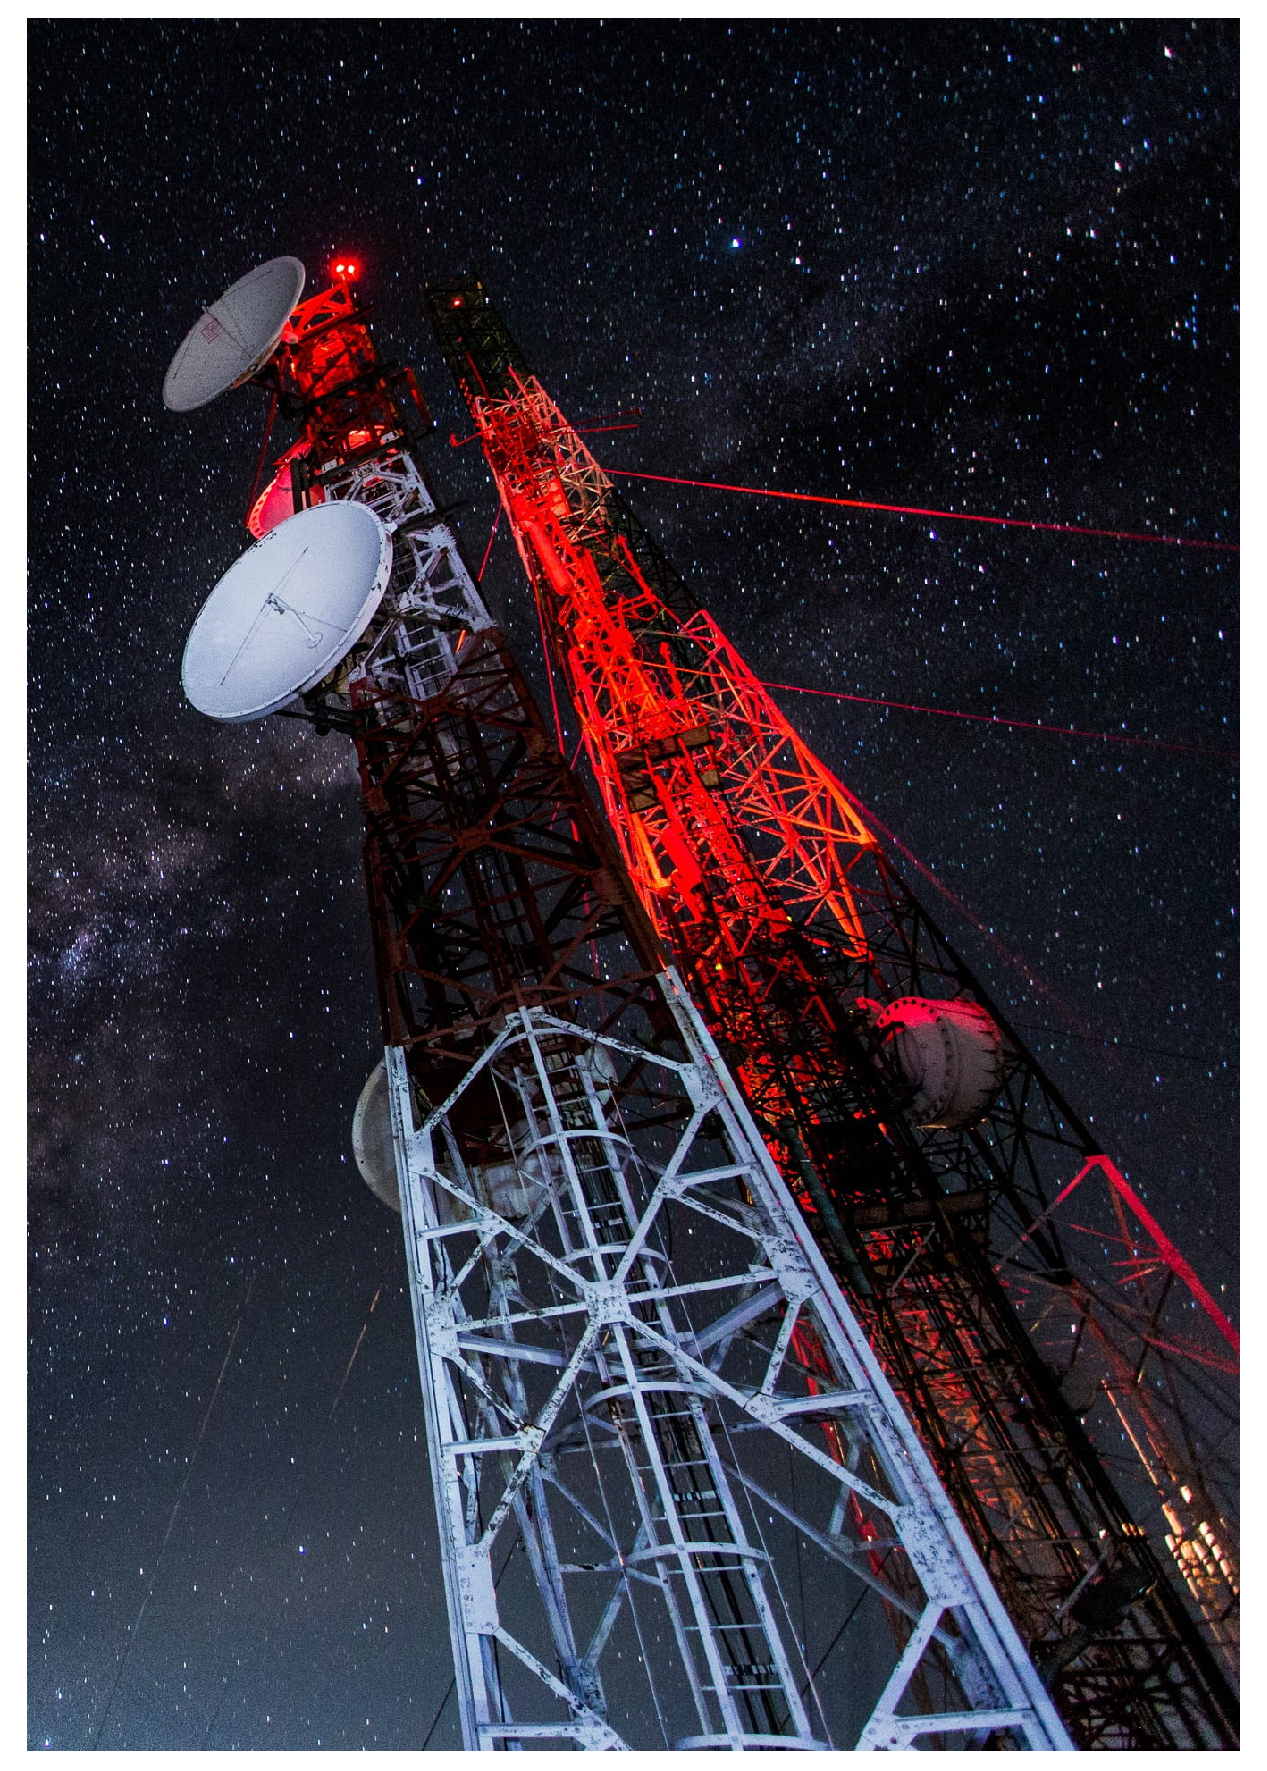
\includegraphics[width=\paperwidth]{background1.pdf}};%here you change your bookcover background
\draw (current page.center) node [fill=ocre!30!white,fill opacity=0.6,text opacity=1,inner sep=1cm]{\Huge\centering\bfseries\sffamily\parbox[c][][t]{\paperwidth}{\centering Apuntes sobre Telecomunicaciones\\[15pt] % Book title
{\Large Notas de un estudiante}\\[20pt] % Subtitle
{\huge Jose Antonio Hancco M.}}}; % Author name
\end{tikzpicture}
\vfill
\endgroup

%----------------------------------------------------------------------------------------
%	COPYRIGHT PAGE
%----------------------------------------------------------------------------------------

\newpage
~\vfill
\thispagestyle{empty}

\noindent Copyright \copyright\ 2022 Jose Hancco\\ % Copyright notice

\noindent \textsc{Libro libre de usos}\\ % Publisher

\noindent \textsc{https://github.com/Yasperterian}\\ % URL

\noindent Con licencia de Creative Commons Attribution-NonCommercial 3.0 Unported License (la ``Licencia''). No puede usar este archivo excepto de conformidad con la Licencia. Puede obtener una copia de la Licencia en \url{http://creativecommons.org/licenses/by-nc/3.0}. A menos que lo exija la ley aplicable o se acuerde por escrito, el software distribuido bajo la Licencia se distribuye \textsc{``tal cual'', sin garantías ni condiciones de ningún tipo}, ya sea expresa o implícita. Consulte la Licencia para conocer el idioma específico que rige los permisos y las limitaciones en virtud de la Licencia.\\ % License information, replace this with your own license (if any)

\noindent \textit{Primera edición, septiembre 2022} % Printing/edition date

\noindent Si existe algún error, crees que una sección se puede mejorar o dar cualquier tipo de \textit{feedback} acerca del libro no dudes y mándame un correo a \textit{jhanccoma@unsa.edu.pe}, te responderé lo más pronto que pueda y gracias por mejorar este libro de todos y para todos.
%----------------------------------------------------------------------------------------
%Dedicate
%----------------------------------------------------------------------------------------
\clearpage
\begin{center}
    \thispagestyle{empty}
    \vspace*{\fill}
    \textit{Dedicatoria aquí}
    \vspace*{\fill}
\end{center}
\clearpage
%----------------------------------------------------------------------------------------
%	TABLE OF CONTENTS
%----------------------------------------------------------------------------------------

%\usechapterimagefalse % If you don't want to include a chapter image, use this to toggle images off - it can be enabled later with \usechapterimagetrue

\chapterimage{chapter_head_generalindex2.pdf} % Table of contents heading image

\pagestyle{empty} % Disable headers and footers for the following pages

\tableofcontents % Print the table of contents itself

\cleardoublepage % Forces the first chapter to start on an odd page so it's on the right side of the book

\pagestyle{fancy} % Enable headers and footers again
%----------------------------------------------------------------------------------------
%	PART
%----------------------------------------------------------------------------------------
\section*{Libros recomendados:}
\begin{itemize}
\item Fundamentos de circuitos eléctricos\cite{alexander2013fundamentos}
\item Signals and Systems Using MATLAB\cite{chaparro2018signals}
\item Procesamiento de señales analógicas y digitales\cite{ambardar1995analog}
\item Física Para Ciencias E Ingeniería. Vol 1\cite{serway2018fisica1}
\item Física Para Ciencias E Ingeniería. Vol 2\cite{serway2018fisica2}
\item Cálculo de una variable: trascendentes tempranas. 7ma edición \cite{stewart12calculo}
\item Análisis de Fourier\cite{hsu1998analisis}
\item Matemáticas Avanzadas Para Ingeniería\cite{o2014matematicas}
\item Métodos numéricos para ingenieros\cite{chapra2013metodos}
\item Comunicaciones y redes de computadores\cite{stallings2004comunicaciones}
\item Electrónica: teoría de circuitos y dispositivos electrónicos\cite{boylestad1989electronica}
\item Fundamentos de sistemas digitales\cite{floyd2006fundamentos}
\item Tratamiento de señales en tiempo discreto\cite{oppenheim2011tratamiento}
\item Tratamiento digital de señales\cite{proakis2007tratamiento}
\item Sistemas de comunicación digitales y análogos\cite{couchsistemas}
\item Data communication and networking\cite{forouzan2007data}
\item Life Pre-Intermediate 2e\cite{hughes2017life}
\item Redes de computadoras\cite{tanenbaum2012computer}
\item Líneas de transmisión\cite{velalineas1999}
\end{itemize}
%----------------------------------------------------------------------------------------
%	NEW CHAPTER
%----------------------------------------------------------------------------------------
\part{Telecomunicaciones 2}
\chapterimage{chapter_head_T2.pdf} % Chapter heading image

\chapter{Unidad I}

\section{Theorems}\index{Theorems}

This is an example of theorems.

\subsection{Several equations}\index{Theorems!Several Equations}
This is a theorem consisting of several equations.

\begin{theorem}[Name of the theorem]
In $E=\mathbb{R}^n$ all norms are equivalent. It has the properties:
\begin{align}
& \big| ||\mathbf{x}|| - ||\mathbf{y}|| \big|\leq || \mathbf{x}- \mathbf{y}||\\
&  ||\sum_{i=1}^n\mathbf{x}_i||\leq \sum_{i=1}^n||\mathbf{x}_i||\quad\text{where $n$ is a finite integer}
\end{align}
\end{theorem}

\subsection{Single Line}\index{Theorems!Single Line}
This is a theorem consisting of just one line.

\begin{theorem}
A set $\mathcal{D}(G)$ in dense in $L^2(G)$, $|\cdot|_0$. 
\end{theorem}

%------------------------------------------------

\section{Definitions}\index{Definitions}

This is an example of a definition. A definition could be mathematical or it could define a concept.

\begin{definition}[Definition name]
Given a vector space $E$, a norm on $E$ is an application, denoted $||\cdot||$, $E$ in $\mathbb{R}^+=[0,+\infty[$ such that:
\begin{align}
& ||\mathbf{x}||=0\ \Rightarrow\ \mathbf{x}=\mathbf{0}\\
& ||\lambda \mathbf{x}||=|\lambda|\cdot ||\mathbf{x}||\\
& ||\mathbf{x}+\mathbf{y}||\leq ||\mathbf{x}||+||\mathbf{y}||
\end{align}
\end{definition}

%------------------------------------------------

\section{Notations}\index{Notations}

\begin{notation}
Given an open subset $G$ of $\mathbb{R}^n$, the set of functions $\varphi$ are:
\begin{enumerate}
\item Bounded support $G$;
\item Infinitely differentiable;
\end{enumerate}
a vector space is denoted by $\mathcal{D}(G)$. 
\end{notation}

%------------------------------------------------

\section{Remarks}\index{Remarks}

This is an example of a remark.

\begin{remark}
The concepts presented here are now in conventional employment in mathematics. Vector spaces are taken over the field $\mathbb{K}=\mathbb{R}$, however, established properties are easily extended to $\mathbb{K}=\mathbb{C}$.
\end{remark}

%------------------------------------------------

\section{Corollaries}\index{Corollaries}

This is an example of a corollary.

\begin{corollary}[Corollary name]
The concepts presented here are now in conventional employment in mathematics. Vector spaces are taken over the field $\mathbb{K}=\mathbb{R}$, however, established properties are easily extended to $\mathbb{K}=\mathbb{C}$.
\end{corollary}

%------------------------------------------------

\section{Propositions}\index{Propositions}

This is an example of propositions.

\subsection{Several equations}\index{Propositions!Several Equations}

\begin{proposition}[Proposition name]
It has the properties:
\begin{align}
& \big| ||\mathbf{x}|| - ||\mathbf{y}|| \big|\leq || \mathbf{x}- \mathbf{y}||\\
&  ||\sum_{i=1}^n\mathbf{x}_i||\leq \sum_{i=1}^n||\mathbf{x}_i||\quad\text{where $n$ is a finite integer}
\end{align}
\end{proposition}

\subsection{Single Line}\index{Propositions!Single Line}

\begin{proposition} 
Let $f,g\in L^2(G)$; if $\forall \varphi\in\mathcal{D}(G)$, $(f,\varphi)_0=(g,\varphi)_0$ then $f = g$. 
\end{proposition}

%------------------------------------------------

\section{Examples}\index{Examples}

This is an example of examples.

\subsection{Equation and Text}\index{Examples!Equation and Text}

\begin{example}
Let $G=\{x\in\mathbb{R}^2:|x|<3\}$ and denoted by: $x^0=(1,1)$; consider the function:
\begin{equation}
f(x)=\left\{\begin{aligned} & \mathrm{e}^{|x|} & & \text{si $|x-x^0|\leq 1/2$}\\
& 0 & & \text{si $|x-x^0|> 1/2$}\end{aligned}\right.
\end{equation}
\end{example}

\subsection{Paragraph of Text}\index{Examples!Paragraph of Text}

\begin{example}[Example name]
\lipsum[2]
\end{example}

%------------------------------------------------

\section{Exercises}\index{Exercises}

This is an example of an exercise.

\begin{example}
This is a good place to ask a question to test learning progress or further cement ideas into students' minds.
\end{example}

%------------------------------------------------

\section{Problems}\index{Problems}

\begin{problem}
What is the average airspeed velocity of an unladen swallow?
\end{problem}

%------------------------------------------------

\section{Vocabulary}\index{Vocabulary}


\begin{vocabulary}[Word]
Definition of word.
\end{vocabulary}

\section{Table}\index{Table}

\begin{table}[h]
\centering
\begin{tabular}{l l l}
\toprule
\textbf{Treatments} & \textbf{Response 1} & \textbf{Response 2}\\
\midrule
Treatment 1 & 0.0003262 & 0.562 \\
Treatment 2 & 0.0015681 & 0.910 \\
Treatment 3 & 0.0009271 & 0.296 \\
\bottomrule
\end{tabular}
\caption{Table caption}
\label{tab:example} % Unique label used for referencing the table in-text
%\addcontentsline{toc}{table}{Table \ref{tab:example}} % Uncomment to add the table to the table of contents
\end{table}

Referencing Table \ref{tab:example} in-text automatically.

%------------------------------------------------

\section{Figure}\index{Figure}
\begin{figure}[h]
\centering
\includegraphics[scale=0.5]{placeholder.jpg}
\caption{Figure caption}
\label{fig:placeholder} % Unique label used for referencing the figure in-text
%\addcontentsline{toc}{figure}{Figure \ref{fig:placeholder}} % Uncomment to add the figure to the table of contents
\end{figure}

Referencing Figure \ref{fig:placeholder} in-text automatically.
%----------------------------------------------------------------------------------------
%	ANEXOS
%----------------------------------------------------------------------------------------
\part{Anexos}
%---------------------------------------------------------------
% 		ENDING
%---------------------------------------------------------------
\stopcontents[part] % Manually stop the 'part' table of contents here so the previous Part page table of contents doesn't list the following chapters

%----------------------------------------------------------------------------------------
%	BIBLIOGRAPHY
%----------------------------------------------------------------------------------------

\chapterimage{Final2.jpg} % Chapter heading image
\chapterspaceabove{6.75cm} % Whitespace from the top of the page to the chapter title on chapter pages
\chapterspacebelow{7.25cm} % Amount of vertical whitespace from the top margin to the start of the text on chapter pages

%------------------------------------------------
\chapter*{Bibliography}
\markboth{\sffamily\normalsize\bfseries Bibliography}{\sffamily\normalsize\bfseries Bibliography} % Set the page headers to display a Bibliography chapter name
\addcontentsline{toc}{chapter}{\textcolor{ocre}{Bibliography}} % Add a Bibliography heading to the table of contents

\section*{Articles}
\addcontentsline{toc}{section}{Articles} % Add the Articles subheading to the table of contents

%\printbibliography[heading=bibempty,type=article] % Output article bibliography entries

\section*{Books}
\addcontentsline{toc}{section}{Books} % Add the Books subheading to the table of contents

\printbibliography[heading=bibempty,type=book] % Output book bibliography entries
%----------------------------------------------------------------------------------------
%	APPENDICES
%----------------------------------------------------------------------------------------
%
%\chapterimage{Final1.jpg} % Chapter heading image
%\chapterspaceabove{6.75cm} % Whitespace from the top of the page to the chapter title on chapter pages
%\chapterspacebelow{7.25cm} % Amount of vertical whitespace from the top margin to the start of the text on chapter pages
%
%\begin{appendices}
%
%\renewcommand{\chaptername}{Appendix} % Change the chapter name to Appendix, i.e. "Appendix A: Title", instead of "Chapter A: Title" in the headers
%
%%------------------------------------------------
%
%\chapter{Appendix Chapter Title}
%
%\section{Appendix Section Title}
%
%Lorem ipsum dolor sit amet, consectetur adipiscing elit. Aliquam auctor mi risus, quis tempor libero hendrerit at. Duis hendrerit placerat quam et semper. Nam ultricies metus vehicula arcu viverra, vel ullamcorper justo elementum. Pellentesque vel mi ac lectus cursus posuere et nec ex. Fusce quis mauris egestas lacus commodo venenatis. Ut at arcu lectus. Donec et urna nunc. Morbi eu nisl cursus sapien eleifend tincidunt quis quis est. Donec ut orci ex. Praesent ligula enim, ullamcorper non lorem a, ultrices volutpat dolor. Nullam at imperdiet urna. Pellentesque nec velit eget est euismod pretium.
%
%%------------------------------------------------
%
%\chapter{Appendix Chapter Title}
%
%\section{Appendix Section Title}
%
%Lorem ipsum dolor sit amet, consectetur adipiscing elit. Aliquam auctor mi risus, quis tempor libero hendrerit at. Duis hendrerit placerat quam et semper. Nam ultricies metus vehicula arcu viverra, vel ullamcorper justo elementum. Pellentesque vel mi ac lectus cursus posuere et nec ex. Fusce quis mauris egestas lacus commodo venenatis. Ut at arcu lectus. Donec et urna nunc. Morbi eu nisl cursus sapien eleifend tincidunt quis quis est. Donec ut orci ex. Praesent ligula enim, ullamcorper non lorem a, ultrices volutpat dolor. Nullam at imperdiet urna. Pellentesque nec velit eget est euismod pretium.
%
%%------------------------------------------------
%
%\end{appendices}
%----------------------------------------------------------------------------------------
%	INDEX
%----------------------------------------------------------------------------------------

\cleardoublepage % Make sure the index starts on an odd (right side) page
\phantomsection
\setlength{\columnsep}{0.75cm} % Space between the 2 columns of the index
\addcontentsline{toc}{chapter}{\textcolor{ocre}{Index}} % Add an Index heading to the table of contents
\printindex % Output the index
%----------------------------------------------------------------------------------------
%	CHAPTER
%----------------------------------------------------------------------------------------

\end{document}
